%% Template for MLP Coursework 2 / 6 November 2017 

%% Based on  LaTeX template for ICML 2017 - example_paper.tex at 
%%  https://2017.icml.cc/Conferences/2017/StyleAuthorInstructions

\documentclass{article}

\usepackage[T1]{fontenc}
\usepackage{amssymb,amsmath}
\usepackage{txfonts}
\usepackage{microtype}

% For figures
\usepackage{graphicx}
\usepackage{subfigure} 

% For citations
\usepackage{natbib}

% For algorithms
\usepackage{algorithm}
\usepackage{algorithmic}

% the hyperref package is used to produce hyperlinks in the
% resulting PDF.  If this breaks your system, please commend out the
% following usepackage line and replace \usepackage{mlp2017} with
% \usepackage[nohyperref]{mlp2017} below.
\usepackage{hyperref}
\usepackage{url}
\urlstyle{same}

% Packages hyperref and algorithmic misbehave sometimes.  We can fix
% this with the following command.
\newcommand{\theHalgorithm}{\arabic{algorithm}}


% Set up MLP coursework style (based on ICML style)
\usepackage{mlp2017}
\mlptitlerunning{MLP Coursework 2 (\studentNumber)}
\bibliographystyle{icml2017}


\DeclareMathOperator{\softmax}{softmax}
\DeclareMathOperator{\sigmoid}{sigmoid}
\DeclareMathOperator{\sgn}{sgn}
\DeclareMathOperator{\relu}{relu}
\DeclareMathOperator{\lrelu}{lrelu}
\DeclareMathOperator{\elu}{elu}
\DeclareMathOperator{\selu}{selu}
\DeclareMathOperator{\maxout}{maxout}

%% You probably do not need to change anything above this comment

%% REPLACE this with your student number
\def\studentNumber{s1700260}

\begin{document} 

\twocolumn[
\mlptitle{MLP Coursework 2: Learning rules, BatchNorm, and ConvNets}

\centerline{\studentNumber}

\vskip 7mm
]

\begin{abstract} 
As the complexity of neural networks increases to solve more difficult tasks, the former techniques to optimize them fail to do so. This entails the development of new methods to maintain the performance of such neural networks in a good level. One of the components in neural networks under continuous evolution is the learning rule, being Root Mean Square Propagation (RMSProp) and Adaptive Moment Estimation (Adam) two examples of that evolution. Following the same direction, other kinds of techniques for faster learning like Batch Normalization (BN) have been developed as well. However, not just the internal components of neural networks evolve, new types of neural networks have been designed to solve more complex tasks or the same tasks in a better way, Convolutional Neural Networks (CNN) are a salient example. In this report, I present the results and analysis the of experiments using the previous techniques and networks ran over the Extended Modified National Institute of Standards and Technology database (EMNIST).

\end{abstract} 

\section{Introduction}
\label{sec:intro}
The increasing use of neural networks in new and more complex tasks leads to an increase in their complexity which causes previous optimization methods not to fit well, therefore, new methods and alternatives have appeared. Learning rules are one of the components of neural networks that experience this change. As the complexity of a neural network increases, the more difficult is to optimize it with classic learning rules. A more complex network can cause that a simple gradient descent rule reaches a local minima and the optimization of the system stops. This is one of the reasons for the development of new learning methods that allow a continuous optimization of a system.

In addition, when training a machine learning model it is recommended to normalize the input data to make its features comparable and avoid that some of these features have more influence in the system than the rest. However, in the case of neural networks, as the data is propagated across the layers, the original normalization is lost. The reason is that the data is modified by the parameters of every layer which causes a change in its distribution in each one of them. This behaviour has been decribed as Internal Covariate Shift in \citep{ioffe2015batch}; the proposed solution for this problem is BN.

The irruption of neural networks allowed to have a new approach to solve tasks that were already addressed by other machine learning methods. Under this premise, new types of neural networks have appeared to solve similar tasks. CNNs is one of the different systems that can be used to solve previously addressed tasks, being one of their major strength the classification of images tasks.

The experiments I report in this document were ran using the EMNIST database \citep{cohen2017emnist}. EMNIST along with MNIST are subsets of the larger NIST Special Dataset 19. EMNIST has the same conversion process as the MNIST dataset, thus it has 28x28 centered images. EMNIST contains the same 10 digits classes plus 26 lower case letters and 26 upper case letters, which leads to 62 potential classes. However, for the current experiments, the number of classes has been reduced to 47. The reason is to avoid confusions due to the similarity of upper and lower case for the following letters: C, I, J, K, L, M, O, P, S, U, V, W, X, Y and Z. The number of samples in the training, validation, and testing datasets are 100000, 15800 and 15800 respectively. For every experiment, I normalized the data to have zero mean and unit standard deviation.

\section{Baseline systems} 
I used three baseline systems to make comparisons between different learning rules and BN. The baseline systems are composed of three hidden layers, this decision is motivated by the complexity of a network against the task to solve and the amount of training data. In a set of previous experiments ran over MNIST (for coursework 1), I used systems with three hidden layers; I obtained reasonably good results. Therefore, my expectation was to use similar systems and still get favorable results even though the task to solve is more complex since the number of classes is almost five times higher. Additionally, I used a simple stochastic descent rule to optimize them; ReLU activations were used for every hidden layer; the error was calculated using cross-entropy with softmax.

The first system is a fully connected network with dropout strategy to avoid overfitting (discarding half of the values in every layer); this network has 46797 parameters to train. This model is motivated by the fact that randomly discarding values from one layer to the next increases even more the variation of the distribution of the data. The second network is similar to the previous one but does not uses dropout; the number of parameter for this system is 93347. Since the complexity of the second model is higher due to the number of parameters to train (it roughly doubles the number of parameters), L2 regularization has been applied to it to compensate that situation. 

Finally, the third system does not use the raw pixel data from the dataset. Instead, a modification of the features is done; the histogram of gradients (HOG) is calculated for every sample following the configuration described in \citep{banjare2016numeric}. HOG is highly used in computer vision tasks, being the most remarkable one the identification of humans \citep{dalal2005histograms}. This model has 18547 parameters, therefore, its complexity is much lower than the previous two. For this reason, no dropout or regularization techniques are used within it. This system is motivated by the premise stated in the \hyperref[sec:intro]{introduction} regarding different approaches to solving a similar task.

As shown in table~\ref{tab:baseline-systems-table}, the network that uses regularization has the highest accuracy. It is clearly evident that the number of parameters in the baseline systems is correlated to the accuracy (the higher the number of parameters, the higher the accuracy). One might think that is more difficult to train a more complex a network, and the accuracy should be lower as well, which is true to some extent. However, one of the reasons for the success of neural networks is the amount of available data to train them. In this case, there are tens of thousands of samples in the dataset, which, given the results in table~\ref{tab:baseline-systems-table}, have proven to be good enough for the baseline systems.

\begin{table}[tb]
\vskip 3mm
\begin{center}
\begin{small}
\begin{sc}
\begin{tabular}{lcccr}
\hline
\abovespace\belowspace
Network & Number of parameters & Validation accuracy \\
\hline
\abovespace
Regularization	& 93347 & 80.79\% \\
Dropout    		& 46797 & 74.55\% \\
HOG			    & 18547 & 71.51\% \\

\hline
\end{tabular}
\end{sc}
\end{small}
\caption{Number of parameters and accuracy for baseline systems. Hyper-parameters for the systems are learning rate (0.001), batch size (50) and number of epochs (100)}
\label{tab:baseline-systems-table}
\end{center}
\vskip -3mm
\end{table}

\section{Learning rules}
As mentioned previously, one of the problems of learning rules like simple stochastic gradient descent is the high chances to reach local minima, especially when the model increases its complexity. Other drawbacks attained to this kind of approaches is the static learning rate applied to all of the parameters. This causes that all the features of the data set have the same impact on the learning which might not be the best approach since their frequencies and values can have different variances. Moreover, a static learning rate can delay the learning process if it is too small, or it can avoid convergence if it is too high.

A multitude of approaches has emerged to solve the problems mentioned above. I experimented with two popular options: Adam \citep{kingma2014adam} and RMSProp \citep{tieleman2012rmsprop}. Both alternatives are meant to break the invariability of the learning rate by recalling the past gradients for every parameter. In the case of RMSProp, the main idea is to adapt the learning rate according to the previous gradients and the current one. The influence of the gradients of previous iterations is defined as the mean of their squared values; for the current gradient, it is simply its squared value as seen in equation \ref{eq:rmsprop_influence}. The learning rule is then adapted for a given parameter and used to update it at a given iteration as shown in equation \ref{eq:rmsprop_update_param}. The suggested value for $\beta$ is 0.9; the $\epsilon$ parameter is meant to avoid division by zero.

\begin{equation}
	E\lbrack g^2 \rbrack_t = \beta E\lbrack g^2 \rbrack_{t-1} + (1 - \beta) g_t^2
	\label{eq:rmsprop_influence}
\end{equation}

\begin{equation}
	\theta_{t+1} = \theta_t - \frac{\eta}{\sqrt{E\lbrack g^2 \rbrack_t + \epsilon}} g_t
	\label{eq:rmsprop_update_param}
\end{equation}

Adam uses the same strategy of previous gradients as RMSProp, but also adds a momentum influence. The idea of the momentum is similar to the concept from Physics. A simplistic way to understand this phenomenon is when cycling down a hill. At the top of the hill, and assuming the cyclist moves just due to the action of gravity, the momentum is low. However, as the cyclist goes down the hill, his velocity and momentum increases and it is more difficult to stop. The same idea is applied for gradient descent, based on the previous gradients we can update the learning rate to make it bigger as we approach the valley of the function.

Based on the previous the learning rate using Adam is adapted based on two estimates: mean and the variance as shown in equations \ref{eq:adam_mean} and \ref{eq_adam_var} respectively. In the original paper, the authors used a correction strategy to reduce the biases of the mean and variance since they are initialized to zero. However, for the experiments of this report, I avoided that correction. Finally, a single parameter is updated according to equation \ref{eq_adam_update_param}. The suggested values for $\beta_1$ and $\beta_2$ are 0.9 and 0.999 respectively.

\begin{equation}
	m_t = \beta_1 m_{t-1} + (1 - \beta_1) g_t
	\label{eq:adam_mean}
\end{equation}

\begin{equation}
	v_t = \beta_2 v_{t-1} + (1 - \beta_2) g_t^2
	\label{eq_adam_var}
\end{equation}

\begin{equation}
	\theta_{t+1} = \theta_t - \frac{\eta}{\sqrt{v_t} + \epsilon} m_t
	\label{eq_adam_update_param}
\end{equation}

For the experiments, I replace the default learning rule with Adam and RMSProp. Figure \ref{fig:fg_lr} shows the evolution of the validation error for every baseline system using each learning rule. It is clearly evident that the system with HOG had better results with Adam and RMSProp. In both cases, the error is lower than the default approach; moreover, the smallest value is reached before 20 epochs. In regards to the system with L2 regularization, the results are similar. However, the difference is less notorious since the default learning rule reaches the same small error, with a higher number of epochs though. 

The model with dropout shows interesting results. First, Adam still gives good results compared to the two previous networks; however, RMSProp not only does not improve the learning, it makes it worse. One of the reasons for this behaviour may be the fact that with dropout part of the features are randomly discarded; therefore, different subsets of the features are used to update the parameters at every iteration. It seems that Adam counteracts this problem with the momentum influence. These statements are not conclusive and further experiments need to be performed.

\begin{figure*}[tb]
\vskip 5mm
\begin{center}
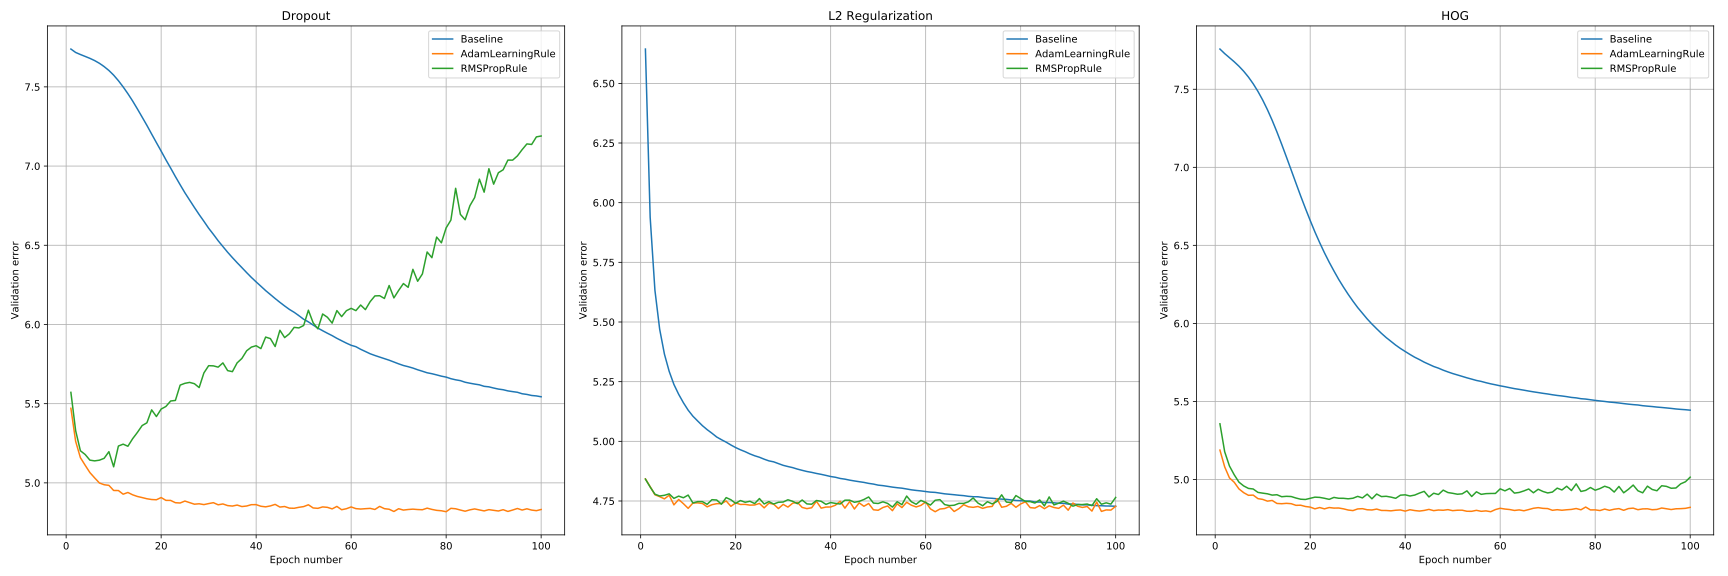
\includegraphics[width=\textwidth,height=4cm]{exp1_metrics}
\caption{Evolution of validation error with Adam and RMSProp for the baseline systems. Hyper-parameters for the systems are learning rate (0.001), batch size (50) and number of epochs (100)}
\label{fig:fg_lr}
\end{center}
\vskip -5mm
\end{figure*}

\section{Batch normalisation}
Batch normalization is defined as an alternative to reduce the effects of internal covariate shift. Due to the changes in the distribution of the input values in every layer, it is difficult to train a network; its parameters have to be carefully initialized and the learning rate has to be small. As stated by its authors, BN allows higher learning rates along with the reduction of the care for initialization strategies for the parameters.  
 
For an affine layer, the forward propagation in batch normalization is defined according to equation \ref{eq_bn_fp}, being $\gamma$ and $\beta$ learnable parameters. The term $\hat{h}$ represents the outputs of the affine layer after normalization as shown in equation \ref{eq_bn_norm}.

\begin{equation}
	y = \gamma \hat{h} + \beta
	\label{eq_bn_fp}
\end{equation}

\begin{equation}
	\hat{h} = \frac{(h - \mu)}{\sqrt{\sigma^2 + \epsilon}}
	\label{eq_bn_norm}
\end{equation}

The backpropagation in batch normalization includes the derivatives of the loss function with respect to the inputs and the derivatives with respect to the parameters $\beta$ and $\gamma$. As depicted in equation \ref{eq_bn_fp}, the output of a batch normalization layer resembles the output of an affine layer. Thus, the gradients with respect to the parameters $\beta$ and $\gamma$ are similar to the gradients with respect to weights and biases in an affine layer which can be seen in equations \ref{eq_bn_gwrt_gamma} and \ref{eq_bn_gwrt_beta}.

\begin{equation}
	\frac{dE}{d\beta_j} = \sum_k 	\frac{dE}{dy_{kj}}
	\label{eq_bn_gwrt_gamma}
\end{equation}

\begin{equation}
	\frac{dE}{d\gamma_j} = \sum_k \lbrack \frac{dE}{dy_{kj}} \frac{h_{kj} - \mu_j}{\sqrt{\sigma_j^2 + \epsilon}} \rbrack
	\label{eq_bn_gwrt_beta}
\end{equation}

Following the chain rule, the derivative with respect to the inputs of a batch normalization layer can be seen in equation \ref{eq_bn_chain}. After unwrapping every derivative in the chain and performing algebraic operations, the final form for the derivate with respect to the inputs is shown in equation \ref{eq_bn_final}

\begin{equation}
	\frac{dE}{dh_{ij}} = \sum_{kl} \frac{dE}{dy_{kl}} \frac{dy_{kl}}{d\hat{h}_{kl}} \frac{d\hat{h}_{kl}}{dh_{ij}}
	\label{eq_bn_chain}
\end{equation}

\begin{equation}
	\frac{dE}{dh_{ij}} = \frac{1}{N} \frac{\gamma_j}{\sqrt{\sigma_j^2 + \epsilon}} (N \frac{dE}{dy_{ij}} - \sum_k \frac{dE}{dy_{kj}} - \frac{h_{ij} - \mu_j}{\sigma_j^2 + \epsilon} \sum_k \frac{dE}{dy_{kj}} (h_{kj} - \mu_j))
	\label{eq_bn_final}
\end{equation}

For the experiments, I simply added a batch normalization layer after every affine layer, the rest of the configuration for every system was the same. As seen in figure \ref{fig:fg_bn}, in terms of accuracy, batch normalization does not present better results; they are remarkably lower than the baseline systems'. The reason for this may be the complexity of the systems; internal covariant shift has bigger effects in large deep neural networks. In those cases, batch normalization plays an important role; however, it seems that the current architectures do not get the benefits of batch normalization.

\begin{figure*}[tb]
\vskip 5mm
\begin{center}
\includegraphics[width=\textwidth,height=4cm]{exp3_metrics}
\caption{Evolution of validation accuracy with batch normalization. Hyper-parameters for the systems are learning rate (0.001), batch size (50) and number of epochs (100)}
\label{fig:fg_bn}
\end{center}
\vskip -5mm
\end{figure*}


\section{Convolutional networks}
Convolutional neural networks irrupted in the scene back in 2012, when they outperformed in the Imagenet Large Scale Visual Recognition Challenge (ILSVRC) \citep{krizhevsky2012imagenet}. Ever since they have become one of the most favourite models for computer vision tasks. There are big differences between fully connected neural networks and CNNs. For simplicity, I will just mention those that are relevant for the experiments described in this report.

Before CNNs, the inputs of a neural network were mainly one-dimensional vectors. This is why systems for tasks that involve images like the digit recognition task uses samples of the data that are continuous sets of pixels. The data of this samples changes its size throughout the network, but it maintains it one-dimensional structure. With CNNs, it is no longer necessary to flatten the images before passing them to the network, they can be passed as 2D matrices.

When an image, defined as a set of 2D feature maps, is passed to a convolutional layer, it is convolved with a set of kernels (also called filters). The output of this operation is usually another set of feature maps, usually with smaller height and width. The image passed to the layer can also be seen as a volume defined by height, width and depth (number of channels); the output corresponds to another volume (slightly smaller in most of the cases) with different dimensions. 

To convolve a set of feature maps, they are split in a set of overlapping patches; the amount of overlapped area is defined by a parameter called stride. All of these patches are convolved with the same kernels, this means that the parameters of the networks are shared between features. In addition, the output feature maps obtained from the convolution layer carry local dependencies of the image. These two key ideas are part of the success of convolutional network layers.

A convolutional layer is usually followed by a max pooling one. The idea of max pooling is to split each 2D feature map into small tiles and discard all the values except the highest one. This is similar to the max out approach used in fully connected networks. The objective here is to reduce overfitting as well.

In the experiments, the forward propagation of a convolution layer is outlined in the algorithm \ref{alg:cnn_fprop}. Key elements of the solution are the \textit{Format} and \textit{FlipAndReshape} routines that are meant to convert the inputs and kernels to a suitable representation to allow matrix multiplications.

\begin{algorithm}[ht]
\begin{algorithmic}
   \STATE {\bfseries Input:} features $x$, kernels $k$, biases $b$
   \STATE {\bfseries Output:} features $y$
   \IF{dimensions ($x$) > dimensions ($k$)}
   \STATE $\hat{x}$ = Format($x$)
   \STATE Cache($\hat{x}$)
   \STATE $\hat{k}$ = FlipAndReshape($k$)
   \STATE $y$ = $\hat{x}$ $\hat{k}$ + $b$
   \ENDIF
\end{algorithmic}
  \caption{Forward propagation for convolution}
  \label{alg:cnn_fprop}
\end{algorithm}

For backward propagation, I calculated the gradients with respect to the inputs following the algorithm \ref{alg:cnn_bprop_param}. This algorithm is as straightforward as the previous one; for the biases, the gradient is calculated similarly to a fully connected layer. In the case of the kernels, I retrieve the data cached in forward propagation, then a matrix multiplication is performed. Finally, the result is represented in a suitable format using the \textit{ReshapeAndFlip} which is the opposite function of \textit{FlipAndReshape} in \ref{alg:cnn_fprop}.

\begin{algorithm}[ht]
\begin{algorithmic}
   \STATE {\bfseries Input:} gradients wrt outputs $y'$
   \STATE {\bfseries Output:} gradienst wrt kernels $k'$, gradients wrt biases $b'$
   \STATE $b'$ = Sum($y'$)
   \STATE $\hat{x}$ = GetFromCache()
   \STATE $k'$ = ReshapeAndFlip($y'$ $\hat{x}$)
\end{algorithmic}
  \caption{Backward propagation for convolution (parameters)}
  \label{alg:cnn_bprop_param}
\end{algorithm}

Finally, the gradient with respect to the inputs is calculated according to algorithm \ref{alg:cnn_bprop_input}. The function of \textit{FlipAndReshape} is the same used in \ref{alg:cnn_fprop}, the \textit{Unformat} routine is meant to convert the result of the matrix multiplication to the same format of the feature maps.

\begin{algorithm}[ht]
\begin{algorithmic}
   \STATE {\bfseries Input:} gradients wrt outputs $y'$, kernels $k$
   \STATE {\bfseries Output:} gradienst wrt inputs $x'$
   \STATE $\hat{k}$ = FlipAndReshape($k$)
   \STATE $x'$ = Unformat($y'$ $\hat{k}$)
\end{algorithmic}
  \caption{Backward propagation for convolution (features)}
  \label{alg:cnn_bprop_input}
\end{algorithm}

The implementation of max pooling is quite straightforward. Given the pool size, the 2D feature maps are split into non-overlapping tiles. In each tile, all the elements are discarded except the maximum value; in this step, a mask is created to determine the positions of the elements with the maximum value in the original feature maps. During backward propagation the mask is used to calculate the gradient with respect to the features; this way the corresponding features elements found in forward propagation are correctly multiplied with the gradient with respects to outputs.

For the experiments, I used two systems; the first one contains one convolutional layer with max pooling of size 2 and one affine layer. The first layer gets a single feature map as input, after convolving it with kernels of size 5 and stride of 1, the output is a set of 5 feature maps. The second model is quite similar to the previous one but adds another convolutional layer after the first one. This second convolution outputs a set of 10 features maps obtained with kernels of the same size (5) and same stride. ReLU activations are used for every layer in each system; the learning rule chosen is Adam (with an initial rate of 0.01) as it demonstrated to have better results in the previous experiments in this report. Only 20 epochs were set due to the high computational cost of this kind of systems; also in the previous experiments, the use of Adam allowed to get good results before that number of epochs, so I expected to have similar results. As described, these models are not very complex since the data to perform the experiments is well formatted and the number of samples is good enough to have considerable results.

The results of the experiments are displayed in \ref{fig:fg_cnn}. One of the first things to highlight is the small error as soon as the model start the training. It is also evident that the models with 2 convolutional layers does a better job in regards to reducing the loss. However, in terms of accuracy, both models seem to do a good job.

\begin{figure}[tb]
\vskip 5mm
\begin{center}
\includegraphics[width=6cm,height=10cm]{expa_metrics}
\caption{Evolution of validation error and accuracy for systems with 1 and convolutional layers . Hyper-parameters for the systems are learning rate (0.01), batch size (50) and number of epochs (20)}
\label{fig:fg_cnn}
\end{center}
\vskip -5mm
\end{figure}

\section{Test results}

n regards to learning and batch normalization; the results show that, overall, the use of Adam as learning rule gives a consistent accuracy through all the systems as shown in table \ref{tab:test_all}. Out of the three systems used in the experiments, the one that uses L2 regularization performs betters than the others for every learning rule and batch normalization. In the other hand, the model with dropout does a slightly better job than the one using HOG when the learning rules are gradient descent and Adam. However, when it comes to RMSProp and batch normalization things change, HOG outputs better results, especially when using RMSProp where its accuracy is more than two times the accuracy of dropout. Finally, the performance of every system with batch normalization went down, especially for dropout where the accuracy was reduced to half compared.

\begin{table}[tb]
\vskip 3mm
\begin{center}
\begin{small}
\begin{sc}
\begin{tabular}{lcccr}
\hline
\abovespace\belowspace
Experiment & L2 Regularization & Dropout & HOG \\
\hline
\abovespace
Baseline	& 78.91\% & 61.46\% & 59.31\% \\
Adam    	& 77.79\% & 75.51\% & 73.48\% \\
RMSProp	 	& 77.39\% & 29.60\% & 69.44\% \\
Batch norm	& 50.43\% & 28.70\% & 39.07\% \\

\hline
\end{tabular}
\end{sc}
\end{small}
\caption{Test accuracy for baseline experiments and their alternatives with Adam and RMSProp learning rules, and batch normalization. Hyper-parameters for the systems are learning rate (0.001), batch size (50) and number of epochs (100)}
\label{tab:test_all}
\end{center}
\vskip -3mm
\end{table}

For CNNs, the experiments show that overall, both systems did a good job; being the model with one convolutional layer a bit better. Compared to the fully connected systems, CNNs did a better job than their best alternative (L2 regularization with gradient descent). It is worth to notice the reduction in the testing performance for the model with two convolutional layers compared to the one with a single convolutional layer. It seems to be a tendency to overfitting when the number of convolutions increases, however, this is not a conclusive statement and further experiments should be performed.

\begin{table}[tb]
\vskip 3mm
\begin{center}
\begin{small}
\begin{sc}
\begin{tabular}{lcccr}
\hline
\abovespace\belowspace
Experiment & Accuracy \\
\hline
\abovespace
1 Convolution	& 83.73\% \\
2 Convolutions 	& 78.96\% \\

\hline
\end{tabular}
\end{sc}
\end{small}
\caption{Test accuracy for CNN experiments. Hyper-parameters for the systems are learning rate (0.01), batch size (50) and number of epochs (20)}
\label{tab:test_cnn}
\end{center}
\vskip -3mm
\end{table}

\section{Conclusions}
\label{sec:concl}

As the complexity of a task increases, some of the optimization methods previously used do no longer fit the needs of new models. In this report, I ran experiments to verify the performance of models using new optimization options over a moderately complex classification task. The results showed that in most of the cases the new learning rules (Adam and RMSProp) improved the behaviour of the networks. However, a seen in the case of dropout and RMSProp, some combinations not just do not improve the performance, they made it worse. For this reason, a careful analysis of the system along with the type and complexity of the task should be done before modify them, otherwise, the results might not be the expected.

In the same line, techniques like batch normalization were developed to reduce the influence of an undesired situation in very complex systems. The fact that this kind of methods has proven to be good for such systems does not mean that they are going to be the best alternative in every case. As shown in the experiments, batch normalization did reduce the performance of the systems. However, I cannot conclude that the small complexity of the networks is the only reason for this result. Other experiments that involve other components of the systems need to be performed in order to get more insights about batch normalization in such low complexity models.

As previously mentioned, a task can be approached from different sides. The experiments showed that CNNs were able to improve the results of the classification task. However, increasing the number of convolutions increases the complexity along with the computational cost. Moreover, it seems that complex CNNs tend to overfit over the training set, nonetheless, further experiments with systems having more convolutional layers need to be performed to confirm this.

Overall, I can say that as the complexity of a task increases, it is possible to use new techniques and systems to replace the old ones that do not behave quite well in the new scenario. However, it is important to keep in mind that these new techniques are not going the solve the problem by themselves. It is the combination of factors and components within a neural network which ultimately defines its behaviour or performance, hence, it is important to make a careful analysis before modifying one component or the entire system.

\bibliography{example-refs}

\end{document} 


% This document was modified from the file originally made available by
% Pat Langley and Andrea Danyluk for ICML-2K. This version was
% created by Lise Getoor and Tobias Scheffer, it was slightly modified  
% from the 2010 version by Thorsten Joachims & Johannes Fuernkranz, 
% slightly modified from the 2009 version by Kiri Wagstaff and 
% Sam Roweis's 2008 version, which is slightly modified from 
% Prasad Tadepalli's 2007 version which is a lightly 
% changed version of the previous year's version by Andrew Moore, 
% which was in turn edited from those of Kristian Kersting and 
% Codrina Lauth. Alex Smola contributed to the algorithmic style files.  
